%! suppress = MissingLabel
\documentclass{article}
\usepackage[T1]{fontenc}
\usepackage[main=english]{babel}
\usepackage{url}
\usepackage{lastpage}
\usepackage{fancyhdr}
\usepackage{graphicx}
\usepackage[a4paper, margin=2cm, footskip=18.3pt]{geometry}
\usepackage{listings}
\usepackage[usenames]{color}

\newcommand{\header} {
    \setlength{\headheight}{30pt}\pagestyle{fancy}
    \fancyhead[L]{\includegraphics[height=20pt]{~/Templates/heig-logo}}\fancyhead[C]{PCO 2023\\ Lab 4}
    \fancyhead[R]{Timothée Van Hove \& Aubry Mangold\\\today}\fancyfoot[C]{}
    \fancyfoot[R]{Page \thepage~sur \pageref{LastPage}}\renewcommand{\footrulewidth}{0.3pt}
}


\definecolor{mygreen}{rgb}{0,0.6,0}
\definecolor{mygray}{rgb}{0.5,0.5,0.5}
\definecolor{mymauve}{rgb}{0.58,0,0.82}

\lstset{frame=tb,
    language=C++,
    aboveskip=3mm,
    belowskip=3mm,
    showstringspaces=false,
    columns=flexible,
    basicstyle={\small\ttfamily},
    numbers=left,
    numberstyle=\tiny\color{mygray},
    keywordstyle=\color{blue},
    commentstyle=\color{mygreen},
    stringstyle=\color{mymauve},
    breaklines=true,
    breakatwhitespace=true,
    tabsize=4
}

\begin{document}
    \header


    \section{Introduction}

    The goal of this lab is to implement the management of shared rail sections in a train simulation. The source code of the simulator and a program boilerplate for the student program are provided. The simulator is a multithreaded program that mocks up the behavior of trains on a rail network, leading to synchronization concerns. The student program must implement the management of at least a shared rail section, the synchronization between the trains at the station and an emergency stop system.


    \section{Analysis}
% Talk about the problems arising from having two trains running on two threads that need to be synchoronized
%    Shared resources
%    Critical sections
%    Synchronization
%    Deadlocks

    In a concurrent system where multiple trains are operated by separate threads, special attention must be paid to synchronization to ensure that all entities can use the network safely without running into one another. Critical sections in this context include shared track sections and stations. The tracks, particularly the shared sections, act as shared resources. Without proper synchronization, both trains could attempt to occupy the same section simultaneously, leading to a collision in the simulation. Deadlocks are a significant risk. With two trains, this could occur if both attempt to enter the same shared section from opposite ends and wait indefinitely for the other to leave. Similar to shared sections, stations are points where special synchronization is needed. Both trains might need to use the station simultaneously.

    To solve the critical sections challenges we are going to use both active waiting to ensure the access to only one train and mutual exclusion to ensure that the shared resources are accessed correctly.


    \section{Conception}
% Talk about how train blocks work in real life TIM: Really necessary?
% Talk about which concepts we've used to solve the problem
% Sections: shared section, station, emergency stop

    \subsection{Shared sections}
    To address station synchronization, we implemented a barrier mechanism. This ensures that trains can only leave the station when it is fully occupied. Additionally, we integrated a priority system within this barrier, giving precedence to the last train arriving at the station to depart first when the barrier is lifted. The synchronization barrier can be implemented using semaphores (which may also act as mutexes) and boolean flags.

    \subsection{Station}
    For managing the shared section, we established a synchronization logic which ensures that while one train occupies this critical section, the other train waits. As soon as the first train exits the section, the waiting train receives clearance to enter. This approach effectively prevents conflicts and ensures safe passage through the shared track section. Similarly to the shared sections, the synchronization logic can be implemented using semaphores and boolean flags.

    \newpage


    \section{Implementation}

    \subsection{Routes}

    The different routes that are implemented in the application are generated by the \texttt{routeFactory} method in the \texttt{cppmain.cpp} file. This method takes a \texttt{RouteType} as a parameter and returns a \texttt{Route} object. The \texttt{RouteType} is an enum that defines the different routes that can be generated. The \texttt{Route} object is a structure that contains the parameters necessary to successfully drive a route, including the station contacts, one or more shared sections or the junctions that need to be set to drive the route. Altough the source code could be refactored to use a more object-oriented approach, it was decided that the current implementation was sufficient for the scope of this lab.

    \subsection{Program startup}

    In the main function, we initialize the model railway system, including setting up the model turnouts based on the selected route. Locomotives A and B are initialized with unique identifiers and predetermined speeds, and their starting positions are determined by the route configuration. Then, two threads launch an instance of the runnable locomotivebehavior class. In this class, the run() method is responsible for dictating the locomotive's actions, encompassing station stops, navigation through shared sections, and responses to track junctions.

    \subsection{Shared sections}
    Synchronization of shared track sections is a critical aspect of our implementation. The \texttt{access()} and \texttt{leave()} methods of the \texttt{Synchro} class ensure that only one train occupies a shared section at any given time, effectively preventing the risk of collisions.

    The access to the shared section a rather classical active wait implementation using a semaphore. A boolean flag signals whether the section is free or occupied. If the section is occupied, the train must wait until the section is released by the other train. The critical section of the method is protected by a mutex to ensure that only one thread at a time my modify the shared variables. If the section is not free, the locomotive must stop before doing it's active wait.

    \begin{lstlisting}[caption={The shared section access routine.}, captionpos=b, label=lst:1]
void access(Locomotive& loco) override {
    mutexSection.acquire();

    if (!isSectionFree) {
        loco.arreter();
        otherIsWaiting = true;
        mutexSection.release();
        sectionSemaphore.acquire(); // Blockingly wait for the section to be free.
        mutexSection.acquire();
        otherIsWaiting = false;
        loco.demarrer();
    }

    isSectionFree = false;
    mutexSection.release();
}
    \end{lstlisting}

    The release of the shared section is quite straightforward. The critical section is protected by a mutex to ensure that only one thread at a time my modify the variables and, if another train is waiting on the section, it is released.

    \begin{lstlisting}[caption={The shared section exit routine.}, captionpos=b, label=lst:2]
void leave(Locomotive& loco) override {
    mutexSection.acquire();
    isSectionFree = true;
    // Give access to the other loco if it is waiting.
    if (otherIsWaiting) {
        sectionSemaphore.release();
    }
    mutexSection.release();
}
    \end{lstlisting}

    \subsection{Station}

    To ensure orderly operations in the station, we implemented a barrier mechanism. This approach not only manages station occupancy but also gives priority to the last train that arrives at the station. The barrier uses a boolean status flag that indicates if the station is already occupied or not. The reading and writing to the flag are protected by a mutex. If the current thread is not the last trained arrived in the section, it will blockingly wait for the second train to arrive using a semaphore. Once the second train has arrived, the related thread takes a 5 second sleep and then gives itself priority on the shared section by calling the \texttt{access()} method and setting its priority to 0 (highest priority). Once the priority is set the arriving thread releases the other thread, at which point both locomotives can resume their routine.

    \begin{lstlisting}[caption={The shared section station synchronization routine.}, captionpos=b, label=lst:3]
        void stopAtStation(Locomotive& loco) override {

            // If the station is empty, stop the loco and set the station to occupied.
            mutexStation.acquire();
            if (!isStationOccupied) {
                isStationOccupied = true;
                mutexStation.release();
                loco.arreter();

                // Wait to be released by the last arrived loco.
                stationSemaphore.acquire();

                // Set the priority
                loco.priority = 1;
                loco.demarrer();
            } else {
                // If the station is occupied, wait for 5 seconds and have the last
                // arrived loco start first by already giving it access to the shared section.
                isStationOccupied = false;
                loco.arreter();
                PcoThread::usleep(5e6);

                // Give access to the shared section before releasing other locos so
                // that we're sure it can't be acquired by another loco.
                access(loco);

                // Release the semaphore to signal the first loco that it may continue.
                stationSemaphore.release();

                // Set the loco to the highest priority and restart it.
                // Note: this is useful in the LocoBehavior::run() while loop in order to avoid the
                // prioritized loco trying to acquire the shared section again.
                loco.priority = 0;
                loco.demarrer();
                mutexStation.release();
            }
        }
    \end{lstlisting}

    \subsection{Emergency stop}

    An emergency stop functionality is implemented. This function can be invoked to immediately halt both locomotives, setting their speeds to zero and ensuring an instantaneous stop.

    \begin{lstlisting}[caption={The emergenty stop routine.}, captionpos=b, label=lst:4]
void emergency_stop() {
    locoA.arreter();
    locoB.arreter();
    locoA.fixerVitesse(0);
    locoB.fixerVitesse(0);
}
    \end{lstlisting}

    \subsection{Program exit}

    The simulation runs continuously with the locomotives checking if the shared sections can be accessed and -- if not -- waiting to be able to access it. Only the activation of the emergency stop brings the operation to a halt, but without closing the window. The simulation is gracefully terminated upon the activation of the \textit{close} button, ensuring the proper shutdown of all threads and the safe state of the train model system.


    \section{Tests}

    \subsection{Shared section}
    % Describe the tests we've done to ensure the correctness of our implementation. This section is worth some points.
    The testing of the train simulation system is conducted in a series of different routes to ensure the robustness and reliability of the implementation. These tests were designed to cover a wide range of scenarios, each introducing different complexities and challenges.

    \begin{enumerate}
        \item \textbf{Provided train route:} Initially, we tested the system using the provided default train route. This served as a baseline to verify the fundamental functionality of our implementation, including basic movement of the trains and basic synchronization in shared sections and at stations. The related configuration is \texttt{RouteName::ROUTE\_1}.

        \item \textbf{Route with only a station and a shared section:} We tested a minimalist route that included only a station and a shared section. This scenario allowed us to test that a train behaves correctly, even when it must handle both the shared section and the station at once. The related configuration is \texttt{RouteName::ROUTE\_2}.

        \item \textbf{Route with a shared section right before the station:} Another scenario placed the shared section right before the station. This setup was aimed to test the system's handling of the synchronization mechanism when trains transition quickly from a shared section to a station stop. The related configuration is \texttt{RouteName::ROUTE\_3}.

        \item \textbf{Route with a shared section separated from the Station:} A route where the shared section was separated from the station by a few blocks was also tested. This scenario was aimed at evaluating the system under a more spread-out configuration, ensuring that our synchronization logic remained effective. The related configuration is \texttt{RouteName::ROUTE\_4}.

        \item \textbf{Route with two shared sections:} Going further, we introduced a route featuring two shared sections. This more complex scenario tested the system's capability to manage multiple critical sections simultaneously, ensuring that each train could access and leave these sections and without conflicts or deadlocks. The related configuration is \texttt{RouteName::ROUTE\_5}.

    \end{enumerate}

    \subsection{Station synchronization}

    We validated that the last train to enter the station was the first one to leave the station. Furthermore, we've validated that the locomotive that has to wait in the station doesn't hiccup while starting (it must start and stop to wait to access the shared section in a smooth fasion).

    \subsection*{Emergency stop}

    We tested the emergency stop in different scenarios with the inertia of the model taken into account:
    \begin{itemize}
        \item Just before the station. Inertia makes the train enter the station, which correctly triggers the \texttt{stopAtStation} routine, but the trains stay still even though being allowed to leave.
        \item Just before the critical section warning contact. Inertia makes the train acquire the section and correctly sets the boolean flag indicating that the section is busy. The train does not restart as a result of acquiring the section.
        \item When only one train is the station.
        \item When both trains are outside the station.
        \item When both trains are outside the critical section.
    \end{itemize}


    \section{Conclusion}

    In conclusion, the train simulation system successfully demonstrates the application of concurrent programming principles to a complex, real-world scenario. By employing semaphores and synchronization techniques, we effectively managed shared resources and ensured safe, conflict-free operation of the two trains on a single track system. The diverse testing scenarios further validate the robustness of the proposed implementation.

    The synchronization techniques used in this lab may easily be extended to accommodate shared sections with an indefinite amount of entry and exit paths.

    \appendix

    \newpage


    \section*{Appendix}
    \section{Train routes}
    \begin{figure}[!htb]
        \centering
        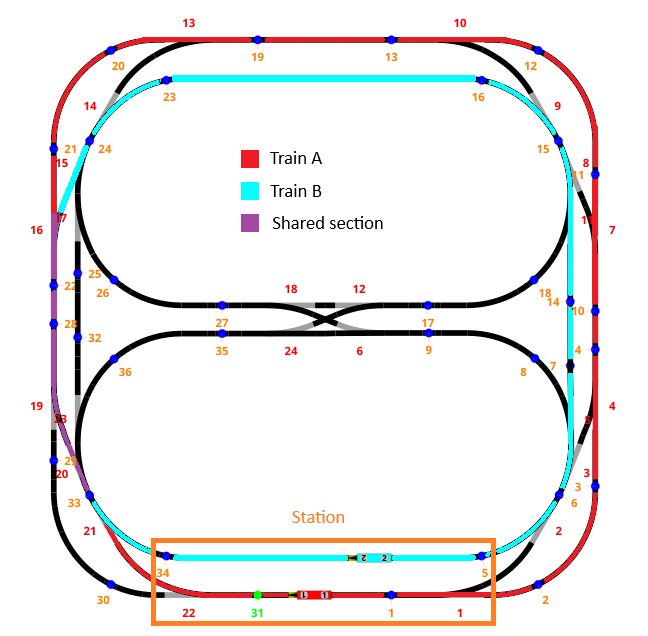
\includegraphics[width=0.6\textwidth]{./doc/assets/Route_1}
        \caption{Train route 1}
    \end{figure}
    \begin{figure}[!htb]
        \centering
        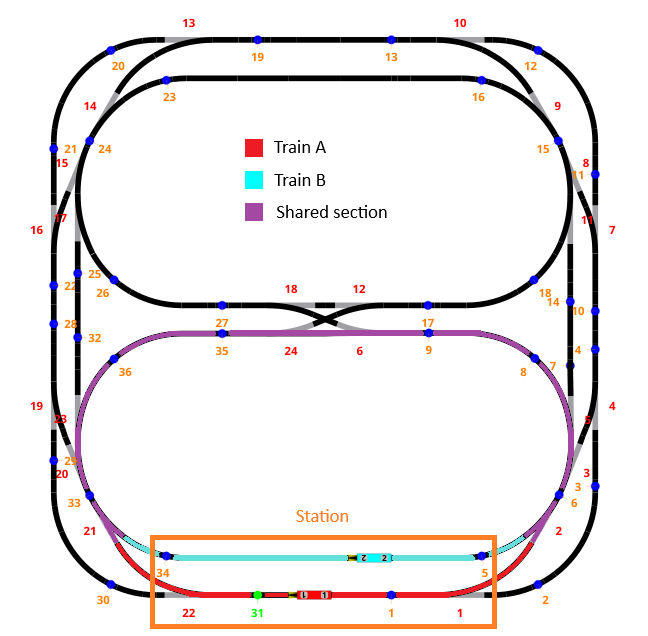
\includegraphics[width=0.6\textwidth]{./doc/assets/Route_2}
        \caption{Train route 2}
    \end{figure}
        \begin{figure}[!htb]
        \centering
        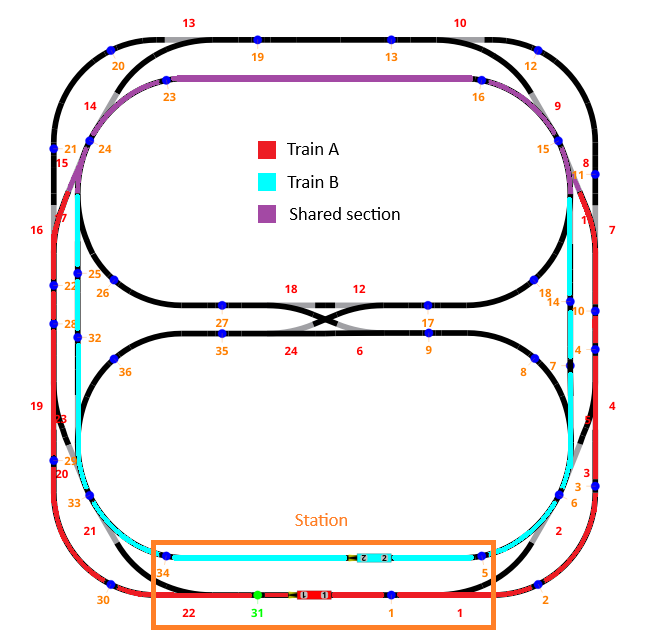
\includegraphics[width=0.6\textwidth]{./doc/assets/Route_3}
        \caption{Train route 3}
    \end{figure}
        \begin{figure}[!htb]
        \centering
        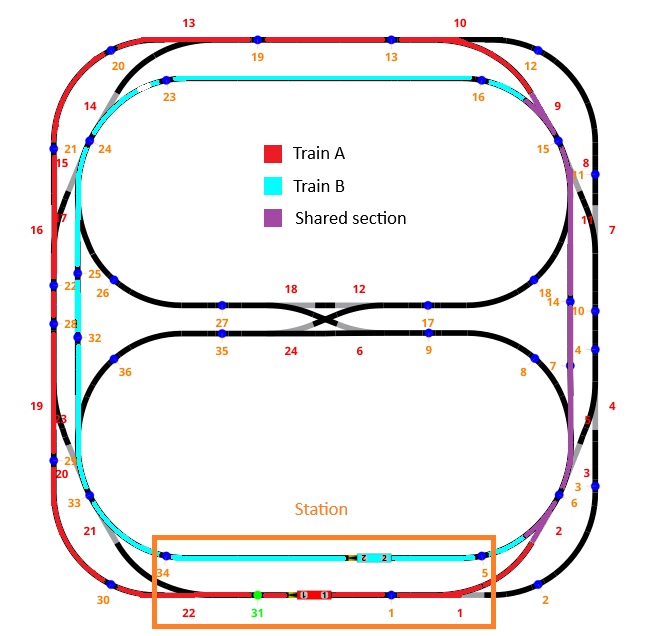
\includegraphics[width=0.6\textwidth]{./doc/assets/Route_4}
        \caption{Train route 4}
    \end{figure}
        \begin{figure}[!htb]
        \centering
        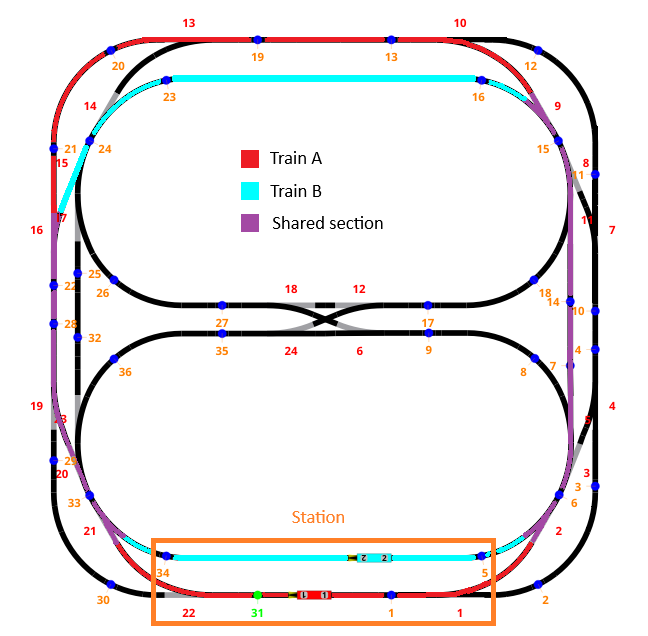
\includegraphics[width=0.6\textwidth]{./doc/assets/Route_5}
        \caption{Train route 5}
    \end{figure}

\end{document}
